
\title{\pkg{tvReg}: Time-varying Coefficients in Multi-Equation Regression in R}
\author{by Isabel Casas and Rub\'{e}n Fern\'andez-Casal}
\maketitle
\abstract{
This article explains the usage of R package \CRANpkg{tvReg}, publicly available
for download from the Comprehensive R Archive Network, via its application to economic and finance problems. The six basic functions in this package cover the kernel estimation of semiparametric panel data, seemingly unrelated equations, vector autoregressive, impulse response, and linear regression models whose coefficients may vary with time or any random variable. Moreover, this package provides methods for the graphical display of results, forecast, prediction, extraction of the residuals and fitted values, bandwidth selection and nonparametric estimation of the time-varying variance-covariance matrix of the error term. Applications to risk management, portfolio management, asset management and monetary policy are used as examples of these functions usage.
}


\section{Introduction}

A very popular research area has been brewing in the field of kernel smoothing statistics applied to linear models with time-varying coefficients. In econometrics, \citet{Robinson1989} was the first to analyse these models for linear regressions with time-varying coefficients and stationary variables. Since then, this literature has extended to models with fewer restrictions in the dependence of the variables to models with time dependence in the error term and to multi-equation models. Although these models are potentially applicable to a large number of areas, no comprehensive computational implementation is, to our knowledge, formally available in any of the commercial programming languages. The package \pkg{tvReg} contains the aforementioned functionality, input and output interface, and user-friendly documentation.

Parametric multi-equation linear models have increased in popularity in the last decades due to an increase in access to multiple datasets. Their application extends to, perhaps, every field of quantitative research. Just to mention some, they are found in biostatistics, finance, economics, business, climate, linguistics, psychology, engineering and oceanography. Panel linear models (PLM) are widely used to account for the heterogeneity in the cross-section and time dimensions. Seemingly unrelated equations (SURE) and vector autoregressive models (VAR) are the extensions of linear regressions and autoregressive models to the multi-equation framework. Programs with these algorithms are found in all major programming languages. Particularly in R, the package \CRANpkg{plm} \citep{CroissantMillo2018, CroissantMillo2008} contains a comprehensive functionality for panel data models. The package \CRANpkg{systemfit} \citep{systemfit} allows the estimation of coefficients in systems of linear regressions, both with equation error terms correlated among equations (SURE) or uncorrelated. Finally, the package \CRANpkg{vars} \citep{vars} provides the tools to fit VAR models and impulse response functions (IRF). All these functions assume that the coefficients are constant. This assumption might not be true when a time series runs for a long period, and the relationships among variables do change. The package \pkg{tvReg} is relevant in this case.

In comparison to parametric models, the appeal of nonparametric models is their flexibility and robustness to functional form misspecification, with spline-based and kernel-based regression methods being the two main nonparametric estimation techniques, \citep[e.g.][]{Eubank1999}. However, fully nonparametric models are not appropriate when many regressors are in play, as their rate of convergence decreases with the number of regressors, the infamous ``curse of dimensionality''. In the case of cross-section data, a popular alternative to avoid this problem are the generalised additive models (GAM), introduced by \citet{HastieTibshirani1993}. The GAM is a family of semiparametric models that extends parametric linear models by allowing for non-linear relationships of the explanatory variables and still retaining the additive structure of the model. In the case of time-series data, the most suitable alternative to nonparametric models is the linear models whose coefficients change over time or follow the dynamics of another random variable. This functionality is coded in R, within the single-equation framework, in packages \CRANpkg{mgm} \citep{mgm2016}, and \CRANpkg{MARSS} \citep{MARSS}. Package \pkg{tvReg} uses the identical kernel smoothing estimation as package \pkg{mgm} when using a Gaussian kernel to estimate a VAR model with varying coefficients (TVVAR). However, the interpretation of their results is different because they are aimed at different audiences. The \pkg{mgm} focuses in the field of network models, producing network plots to represent relationships between current variables and their lags. Whereas the \pkg{tvReg} focuses in the field of economics where a direct interpretation of the TVVAR coefficients is not meaningful and may be done via the time-varying impulse response function (TVIRF) instead. Models with coefficients varying over time can also be expressed in state space form, which assumes that the coefficients change over time in a determined way for example, as a Brownian motion. These models can be estimated using the Kalman filter or Bayesian techniques, for instance \citep{LiuGuo2019, Primiceri2005}. Packages \pkg{MARSS} and \CRANpkg{bvarsv} \citep{bvarsv} implement this approach based on the \citet{CarterKohn1994} algorithm to estimate the TVVAR. On top of all this and as far as we can tell, the \pkg{tvReg} is the only package containing tools to estimate time-varying coefficients seemingly unrelated equation (TVSURE) and panel linear models (TVPLM) in R. 

Simply, the main objective of the \pkg{tvReg} is to provide tools to estimate and forecast linear models with time-varying coefficients in the framework of kernel smoothing estimation, which may be difficult for the nonspecialised end-user to code. For completion, the \pkg{tvReg} also implements methods for the time-varying coefficients linear model (TVLM) and the time-varying coefficients autoregressive (TVAR) model. Often, these can be estimated using packages \CRANpkg{gam} \citep{Gam2022} and \CRANpkg{mgcv} \citep{Wood2017}, which combine (restricted) marginal likelihood techniques in combination with nonparametric methodologies. However, the advantage of using the \pkg{tvReg} is that it can handle dependency and any kind of distribution in the error term because it combines least squares techniques with nonparametric methodologies. An example of this is shown in Section \nameref{ssec:tvLM}.

Summing up, this paper presents a review of the most common time-varying coefficient linear models studied in the econometrics literature during the last two decades, their estimation using kernel smoothing techniques, the usage of functions and methods in the package \pkg{tvReg}, and their latest applications. Along these lines, Table \ref{tab:structure} offers a glimpse at the \pkg{tvReg} full functionality, displaying a summary of its methods, classes and functions. 

\begin{table}[!ht]
\begin{center}
\begin{tabular}{p{0.08\textwidth}p{0.08\textwidth}p{0.46\textwidth}p{0.24\textwidth}}
\multicolumn{1}{l}{Function}&
\multicolumn{1}{l}{Class}&
\multicolumn{1}{l}{Function and Methods for class} & Based on\\  
\hline
\code{tvPLM} & \code{"tvPLM"} &  \code{tvRE}, \code{tvFE}, \code{coef}, \code{confint}, \code{fitted}, \code{forecast}, \code{plot}, \code{predict},
\code{print}, \code{resid}, \code{summary} &\code{plm::plm}\\
\code{tvSURE} & \code{"tvsure"} & \code{tvGLS}, \code{bw}, \code{coef}, \code{confint}, \code{fitted}, \code{forecast}, \code{plot}, \code{predict},
\code{print}, \code{resid}, \code{summary} & \code{systemfit::systemfit} \\
\code{tvVAR} & \code{"tvvar"} & \code{tvAcoef}, \code{tvBcoef}, \code{tvIRF},  \code{tvOLS}, \code{tvPhi}, \code{tvPsi}, \code{bw}, \code{coef}, \code{confint}, \code{fitted}, \code{forecast}, \code{plot}, \code{predict},
\code{print}, \code{resid}, \code{summary}& \code{vars::VAR}\\
\code{tvIRF} & \code{"tvirf"} &  \code{coef}, \code{confint},  \code{plot}, \code{print}, \code{summary}  & \code{vars::irf} \\
\code{tvLM} & \code{"tvlm"} & \code{tvOLS}, \code{bw}, \code{coef}, \code{confint}, \code{fitted}, \code{forecast}, \code{plot}, \code{predict},
\code{print}, \code{resid}, \code{summary}  & \code{stats::lm}\\
\code{tvAR} & \code{"tvar"} & \code{tvOLS}, \code{bw}, \code{coef}, \code{confint}, \code{fitted}, \code{forecast}, \code{plot}, \code{predict},
\code{print}, \code{resid}, \code{summary}& \code{stats::ar.ols}\\
\hline
\end{tabular}
\end{center}
\caption{Structure of the package \pkg{tvReg}.}
\label{tab:structure}
\end{table}


\section{Multi-equation linear models with time-varying coefficients}\label{sec:multi}

A multi-equation model formed by a set of linear models is defined when each equation has its own dependent variable and possible different regressors. Seemingly unrelated equations, panel data models and vector autoregressive models are included in this category.

\subsection{Time-varying coefficients SURE} \label{sec:sure}
The SURE was proposed by \citet{Zellner1962} and is referred to as the seemingly unrelated equations model (SURE). The SURE model is useful to exploit the correlation structure between the error terms of each equation. Suppose that there are $N$ linear regressions of different dependent variables,
\begin{eqnarray}
\label{eq:tvsure} Y_{t} = X_t \beta(z_t)+U_{t} \quad
i=1,\ldots,N\quad t=1,\ldots ,T,
\end{eqnarray}
where $Y_{t}=(y_{1t}\ldots y_{Nt})^\top$ with $y_{i} = (y_{i1}, \ldots, y_{iT})^\top$ denotes the values over the recorded time period of the $i-\mbox{th}$ dependent variable. Each equation in (\ref{eq:tvsure}) may have a different number of exogenous variables, $p_{i}$. The regressors matrix,  $X_t=diag(x_{1t}\ldots x_{Nt})$ with $X_{i}=( x_{i1},\ldots,x_{ip_{i}})$ for equation $i$ and $\beta_{z_t}=( \beta_{1}(z_t)^\top,...,\beta_{N}(z_t)^\top)^\top$ is a vector of order $P = p_1+p_2+ \ldots+p_N$. The error vector, $U_{t}=(u_{1t}\ldots u_{Nt})^\top$,  has zero mean and  covariance matrix $\mathbb{E}(U_tU^\top_t)=\Sigma_t$ with elements $\sigma_{ii^\prime t}$.

It is important to differentiate between two types of smoothing variables: 1) $z_t = \tau = t/T$ is the rescaled time with $\tau \in [0, 1]$, and 2) $z_t$ is the value at time $t$ of the random variable $Z = \{z_t\}_{t=1}^T$. In other words, time-varying coefficients may be defined as unknown functions of time, $\beta(z_t)= f(\tau)$, or as unknown functions of a random variable, $\beta(z_t) = f(z_t)$. The estimation of the TVSURE has been studied by \citet{Hendersonetal2015} when for a random $z_t$ and by \citet{Orbeetal2005} and \citet{Casasetal2019a} for $z_t = \tau$. These estimators are consistent and asymptotically normal under certain assumptions on the size of the bandwidth, kernel regularity and error moments, and dependency. Details are left out of this text as can be easily found in the related literature.

The estimation of system (\ref{eq:tvsure}) may be done separately for each equation as if there is no correlation in the error term across equations, i.e. system (\ref{eq:tvsure}) has a total of $N$ different TVLM with possibly $N$ different bandwidths, $b_i$. In this case, the time-varying coefficients are obtained by combining the ordinary least squares (OLS) and the local polynomial kernel estimator, which is extensively studied in \citet{FanGijbels1996}. The result is the time-varying OLS denoted by TVOLS herein. Two versions of this estimator are implemented in \pkg{tvReg}: i) the TVOLS that uses the local constant (\emph{lc}) kernel method, also known as the Nadaraya-Watson estimator; and ii) the TVOLS which uses the local linear (\emph{ll}) method. Focussing in the single equation $i$, and assuming that $\beta_i(\cdot)$ is twice differentiable, an approximation of $\beta_i(z_t)$ around $z$ is given by the Taylor rule, $\beta_i(z_t) \approx \beta_i(z) + \beta_i^{(1)}(z) (z_t -z)$, where $\beta_i^{(1)}(z) = d\beta_i(z)/dz$ is its first derivative. The estimates resolve the following minimisation:
$$
(\hat \beta_i(z_t), \hat \beta_i^{(1)}(z_t))= \arg \min_{\theta_0, \theta_1} \sum_{t=1}^T \left[ y_i - X_i^\top \theta_0 - (z_t -z) X_i^\top\theta_1\right]^2 K_{b_i}(z_t -z). 
$$
Roughly, these methodologies fit a set of weighted local regressions with an optimally chosen window size. The size of these windows is given by the bandwidth $b_i$, and the weights are given by $K_{b_i}(z_t -z)= b_i^{-1} K(\frac{z_t-z}{b_i})$, for a kernel function $K(\cdot)$. The local linear estimator general expression is
\begin{equation}
\left(\begin{array}{c} \hat\beta_{i}(z_t)\\
\hat\beta_{i}^{(1)}(z_t) \end{array}\right) =
\left (\begin{array}{cc} S_{T,0}(z_t) & {S^\top_{T,1}}(z_t)\\
S_{T,1}(z_t) & S_{T,2}(z_t)\end{array}\right)^{-1} \left (\begin{array}{c} T_{T,0}(z_t) \\
T_{T,1}(z_t)\end{array}\right)
\label{eq:tvols}
\end{equation}
with
\begin{align*}
S_{T, s}(z_t) = &\frac{1}{T}\sum_{i=1}^T X_i^\top X_i (z_i -z_t)^s K\left(\frac{z_i -z_t}{b_i}\right) \\
T_{T, s}(z_t) = &\frac{1}{T}\sum_{i=1}^T X_i^{\top} (z_i - z_t)^s K\left(\frac{z_i -z_t}{b_i}\right) y_i
\end{align*}
and $s= 0, 1, 2$. The particular case of the local constant estimator is calculated by $\hat\beta_{i,t} = S_{T,0}^{-1}(z_t) T_{T, 0} (z_t)$ and it is only necessary that $\beta_i(\cdot)$ has one derivative.

A second option is to use the correlation matrix of the error term in the estimation of system (\ref{eq:tvsure}). This is called the time-varying generalised least squares (TVGLS) estimation. Its mathematical expression is the same as (\ref{eq:tvols}) with the following matrix components:
\begin{align}
S_{T, s}(z_t) = &\frac{1}{T}\sum_{i=1}^T X_i^{\top} K_{B,it}^{1/2}\Sigma _{i}^{-1} K_{B,it}^{1/2} X_i (Z_i -z_t)^s \nonumber\\
T_{T, s}(z_t) = &\frac{1}{T}\sum_{i=1}^T X_i^{\top} K_{B,it}^{1/2} \Sigma _{i}^{-1} K_{B, it}^{1/2} Y_i (Z_i - z_t)^s,
\label{eq:tvgls}
\end{align}
where $K_{B,it}= diag( K_{b_1,it}, ... , K_{b_N,it})$  and $K_{b_i,it}= (T b_i)^{-1} K((Z_i-z_t)/(T b_i))$ is the matrix of weights introducing smoothness according to the vector of bandwidths, $B=(b_1,\ldots,b_N)^\top$. Note that this minimisation problem accounts for the time-varying structure of the variance-covariance matrix of the errors, $\Sigma_t$. 

The TVGLS assumes that the error variance-covariance matrix is known. In practice, this is unlikely and it must be estimated, resulting in the Feasible TVGLS estimator (TVFGLS). This estimator consists of two steps:
\begin{enumerate} 
\item [Step 1] Estimate $\Sigma_t$ based on the residuals of a line by line estimation (i.e,  when $\Sigma_t$ is the identity matrix). If $\Sigma_t$ is known to be constant, the sample variance-covariance matrix from the residuals is a consistent estimator of it. If $\Sigma_t$ changes over time, a nonparametric estimator such the one explained in Section \nameref{sec:tvCov} is a consistent alternative.
\item [Step 2] Estimate the coefficients of the TVSURE by plugging in $\hat \Sigma_t$ from step 1 into Equation (\ref{eq:tvgls}).
\end{enumerate}

To ensure a good estimation of $\Sigma_t$, the iterative TVFLGS may be used. First, do steps 1-2 as above to obtain the residuals from step 2, and repeat step 2 until the estimates of $\Sigma_t$ converge or the maximum number of iterations is reached. 



\subsection{Time-varying coefficients panel data models}

Panel data linear models (PLM) are a particular case of SURE models with the same variables for each equation but measured for different cross-section units, such as countries, and for different points in time. All equations have the same coefficients apart from the intercept which can be different for different cross-sections. Therefore, the data from all cross-sections can be pooled together. The individual effects, $\alpha_i$, account for the heterogeneity embedded in the cross-section dimension. This package only take into account balanced panel datasets, i.e. with the same number of data points for each cross-section unit. 

Coefficient dynamics can be added to classical PLM models using a time-varying coefficients panel data model, TVPLM. Recent developments in this kind of models can be found in \citet{Sunetal2009, Dongetal2015, Casasetal2019b, Dongetal2018} among others, with general model,
\begin{equation}
y_{it} = \alpha_i  + x_{it}^\top \beta(z_{t}) +u_{it} \quad
i=1,\ldots,N , \quad t = 1, \ldots, T.
\label{eq:tvpanel} 
\end{equation}
Note that the smoothing variable only changes in the time dimension, not like in the SURE model where it changed over $i$ and $t$. The three estimators of Equation (\ref{eq:tvpanel}) in the \pkg{tvReg} are:
\begin{enumerate}
\item The time-varying pooled ordinary least squares (TVPOLS) has the same expression than estimator (\ref{eq:tvols}) with the following terms:
\begin{align}
S_{T, s}(z_t) = & X^{\top} K_{b,t}^* X (Z - z_t)^s \nonumber\\
T_{T, s}(z_t) = &X^{\top} K_{b,t}^* Y (Z - z_t)^s,
\label{eq:tvpols}
\end{align}
where $K_{b, t}^*=  I_N \otimes \mbox{diag}\{K_b(z_1-z_t),\ldots, K_b(z_T-z_t)\}$. Note that it is not possible to ignore the panel structure in the semiparametric model because the coefficients change over time. The consistency and asymptotic normality of this estimator needs the classical assumptions about the kernel and the regularity of the coefficients, available in the related literature. 
\item The time-varying random effects (TVRE) estimator is also given by Equation (\ref{eq:tvpols}) with a non-identity $\Sigma$:
\begin{align}
S_{T, s}(z_t) = &X^{\top} K_{b,t}^{*1/2} \Sigma_t^{-1} K_{b,t}^{*1/2} X (Z - z_t)^s \nonumber\\
T_{T, s}(z_t) = &K_{b,t}^{*1/2} \Sigma_t^{-1} K_{b,t}^{*1/2}Y(Z - z_t)^s.
\label{eq:tvRE}
\end{align}
Note that this is a simpler case of (\ref{eq:tvgls}) with the same bandwidth for all equations. The variance-covariance matrix is estimated in the same way using the residuals from the TVPOLS and it may be an iterative algorithm until convergence of the coefficients.
\item The time-varying fixed effects (TVFE) estimator. Unfortunately, the transformation for the within estimation does not work in the time-varying coefficients model because the coefficients depend on time \citep[][explain the issue in detail]{Sunetal2009}. Therefore, it is necessary to make the assumption that  $\sum_{i=1}^N \alpha_i=0$ for identification. The terms in the TVFE estimator are:
\begin{align}
S_{T, s}(z_t) = &X^{\top} W_{b,t} X (Z - z_t)^s \nonumber\\
T_{T, s}(z_t) = &X^{\top} W_{b,t} Y (Z - z_t)^s,
\label{eq:tvFE}
\end{align}
where $W_{b,t}=D_{t}^\top K_{b, t}^*D_{t}$, $D_{t}=I_{NT} -  D(D^\top K_{b, t}^* D)^{-1} D^\top K_{b,t}^*$, $D=(-1_{N-1},I_{N-1})^\top \otimes 1_T$, and $1_k$ is the unity vector of length $k$. The fixed effects are given by, $\hat \alpha = (D^\top K_{b,t}^*D)^{-1}D^\top K_{b,t}^*(Y - X^\top \beta)$. Finally, $\hat \alpha_i = \frac{1}{T} \sum_{t=1}^T \alpha_{it}$ for $i= 2, \ldots, N$.
\end{enumerate}


\subsection{Time-varying coefficient VAR model}

Macroeconomic econometrics experienced a revolution when \citet{Sims1980} presented the vector autoregressive (VAR) model: a new way of summarising relationships among several variables while getting around the problem of endogeneity of structural models. The VAR model has lagged values of the dependent variable, $y_t$, as regressors to which further exogenous variables can be added as regressors. Unless the model is constrained, all variables are the same for every equation, which simplifies the algebra. The model coefficients and variance-covariance matrix may be estimated by maximum likelihood, OLS or GLS. VAR coefficients and the variance-covariance matrix do not have a direct economic interpretation. However, it is possible to use them to recover a structural model by imposing a number of restrictions and so analyse the transmission of a shock, for example, a new monetary policy, to the macroeconomy using the impulse response function (IRF). \citet{Lutkepohl2005} dive into the theoretical properties of these models in detail.

The TVVAR($p$) is an $N$-dimensional system of time-varying autoregressive processes of order $p$ like
\begin{equation}
Y_{t}= A_{0,t}+ A_{1,t} Y_{t-1} + \ldots+ A_{p,t} Y_{t-p} + U_t, \ \  t= 1, 2,\ldots, T.
\label{eq:tvvar}
\end{equation}
In Equation (\ref{eq:tvvar}), $Y_t=(y_{1t}, \ldots, y_{Nt})^\top$ and coefficient matrices at each point in time $A_{j,t}=(a_{1t}^j, \ldots, a_{Nt}^j)$, $j=1, \ldots, p$ are of dimension $N\times N$. Then, notation $A_{j,t}$ means that the elements of this matrix are unknown functions of either the rescaled time value, $\tau$, or of a random variable at time $t$.  The innovation, $U_t=(u_{1t}, \ldots, u_{Nt})$, is an $N$-dimensional identically distributed random variable with $E(U_t) = 0$ and possibly a time-varying positive definite variance-covariance matrix, $E(U_t U_s^\top) =  \Sigma_t, \mbox{ for } t=s,  E(U_t U_s^\top)=0 \mbox{ otherwise}$. Here, matrix $A_{j, t}$ is a function of $\tau$, then process (\ref{eq:tvvar}) is locally stationary in the sense of \citet{Dahlhaus1997}, which occurs when the functions in matrices $A_{j, t}$ are constant or change smoothly over time. Then, process (\ref{eq:tvvar}) at time $t$ has a well defined unique solution given by the Wold representation,
\begin{equation}
\bar y_t = \sum_{j = 0}^\infty \Phi_{j, t}{U}_{t-j},
\label{eq:6}
\end{equation}
such that  $|Y_t - \bar y_t|\rightarrow 0$ almost surely. Matrix $\Phi_{0, t} = I_N$ and matrix $\Phi_{s,t}= \sum_{j=1}^s \Phi_{s-j,t} A_{j,t}$ for horizons $s = 1, 2,\ldots$ As for the constant model, $\Phi_{s,t}$ are the time-varying coefficient matrices of the impulse response function (TVIRF). Its element $(t, i, j)$ may be interpreted as the expected response of $y_{i, t+s}$ to an exogenous shock of $y_{j,t}$ ceteris paribus lags of $y_t$ when the innovations are orthogonal. Otherwise, an orthogonal TVIRF can be found as $\Psi_{j,t} = \Phi_{j,t} P_t$ for $\Sigma_t = P_t P_t^\top$, the Cholesky decomposition of $\Sigma_t$ at time $t$. More theoretical details in \cite{Yanetal2021}.

In the macroeconomic literature, the Bayesian estimation of process (\ref{eq:tvvar}) has attracted a lot of attention in recent years driven by results in \citet{CogleySargent2005, Primiceri2005} and \citet{Kapetaniosetal2012}. In their approach, the coefficients are assumed to follow a random walk. Recently, \citet{Kapetaniosetal2016} studied the inference of the local constant estimator of a TVVAR($p$) for large sets, and they found an increase in the forecast accuracy in comparison to the forecast accuracy of the VAR($p$).

\section{Standard usage of \code{tvSURE}}
\label{ssec:tvsure}
The main argument of this function is a list of formulas, one for each equation. The \code{formula} follows the format of \code{formula} in the package \pkg{systemfit}, which implements estimators of parametric multi-equation models with constant coefficients. The \code{tvSURE} wraps the \code{tvOLS} and \code{tvGLS} methods to estimate the coefficients of system (\ref{eq:tvsure}). The \code{tvOLS} method is used by default, calculating estimates for each equation independently with different bandwidths, \code{bw}. The user is able to enter a set of bandwidths or a single bandwidth to be used in the estimation instead. The \code{tvGLS} method has argument \code{Sigma} where a known variance-covariance matrix of the error can be entered in Equation (\ref{eq:tvgls}). Otherwise, if \code{Sigma = NULL}, the variance-covariance matrix $\Sigma_t$ is estimated using function \code{tvCov}, which is discussed in Section \nameref{sec:tvCov}.

In addition to \code{formula}, function \code{tvSURE} has other arguments to control and choose the desired estimation procedure:

\begin{description}
\item[Smoothing random variable]\hfill\\
All methods assume by default that the coefficients are unknown functions of $\tau = t/T$ and therefore argument \code{z} is set to \code{NULL}. The user can modify this setting by entering a numeric vector in argument \code{z} with the values of the random smoothing variable over the corresponding time period. Note that the current version only allows one single smoothing random variable, \code{z}, common for all equations; and balanced panels.
\item[Bandwidth] \hfill\\ When argument \code{bw} is set to \code{NULL}, it is automatically selected by leave-one-out cross-validation. It is possible to select it by leave-$k$-out cross-validation \citep{ChuMarron1991} by setting argument \code{cv.block = k} (\code{k=0} by default). This minimisation can be slow for large datasets, and it should be avoided if the user knows an appropriate value of the bandwidth for the required problem. 
\item[Kernel type]\hfill\\ The three choices for this argument are  \code{tkernel = "Triweight"} (default), \code{tkernel = "Epa"} and \code{tkernel = "Gaussian"}. The first two options refer to the Triweight and Epanechnikov kernels, which are compact in [-1, 1]. The authors recommend the use of either of those two instead of the Gaussian kernel which, in general, requires more calculations.
\item [Degree of local polynomial]\hfill\\
The default estimation methodology is the Nadaraya-Watson or local constant, which is set as  (\code{est = "lc"}) and it fits a constant at each interval defined by the bandwidth. The argument \code{est = "ll"} can be chosen to perform a local linear estimation (i.e., to fit a polynomial of order 1).
\item [Singular fit] \hfill\\
The \code{tvOLS} method used in the estimation wraps the \code{lm.wfit} method, which at default allows the fitting of a low-rank model, and the estimation coefficients can be \emph{NA}s. The user can change the argument \code{singular.ok} to \code{FALSE}, so that the program stops in case of a low-rank model.
\end{description}
 
The user can restrict certain coefficients in the TVSURE model using arguments \code{R} and \code{r}. Note that the restriction is done by setting those coefficients to a constant. Furthermore, argument \code{method} defines the type of estimator to be used. The possible choices in argument \code{method} are:

\begin{enumerate}
\item  \code{"tvOLS"} for a line by line estimation, i.e, with $\Sigma$ the identity matrix. 
\item  \code{"tvGLS"} to estimate the coefficients of the system using $\Sigma_t$, for which the user must enter it in argument \code{Sigma}. Argument \code{Sigma} takes either a symmetric matrix or an array. If \code{Sigma} is a matrix (constant over time) then it must have dimensions \emph{neq} $\times$ \emph{neq}, where \emph{neq} is the number of equations in the system. If $\Sigma_t$ changes with time, then argument \code{Sigma} is an array of dimension \emph{neq} $\times$ \emph{neq} $\times$ \emph{obs}, where the last dimension measures the number of time observations. Note that if the user enters a diagonal variance-covariance matrix with diagonal values different from one, then a time-varying weighted least squares is performed. If \code{method ="tvGLS"} is entered but \code{Sigma = NULL}, then \code{tvSURE} is fitted as if \code{method = "tvOLS"} and a warning is issued.
\item \code{"tvFGLS"} to estimate the coefficients of the system using an estimate of $\Sigma_t$. By default, only one iteration is performed in the estimation, unless argument \code{control} indicates otherwise. The user can choose the maximum number of iterations or the level of tolerance in the estimation of $\Sigma_t$. See example the below for details.
\end{enumerate}

The package \pkg{systemfit} contains the \code{Kmenta} dataset, which was first described in \citet{Kmenta1986}, to show the usage of the function \code{systemfit} to fit SURE models. This example has two equations: i) a demand equation, which explains how food consumption per capita, \code{consump}, depends on the ratio of food price, \code{price}; and disposable income, \code{income}; and ii) a supply equation, which shows how consumption depends on \code{price}, ratio prices received by farmers to general consumer prices, \code{farmPrice}; and  a possible time trend, \code{trend}. Mathematically, this SURE model is
\begin{align}
consump_t = &\beta_{10} + \beta_{11} price_t + \beta_{12} income_t  + u_{1t}\nonumber\\
consump_t = &\beta_{20} + \beta_{21} price_t+ \beta_{22} farmPrice_t  +\beta_{23} t+  u_{2t}.
\label{eq:Kmenta}
\end{align}
The code below defines the system of equations using two \code{formula} calls which are put into a \code{"list"}. 

%%
%% Example 1: Usage of the tvSURE formula
%%
\begin{Schunk}
\begin{Sinput}
> data("Kmenta", package = "systemfit")
> eqDemand <- consump ~ price + income
> eqSupply <- consump ~ price + farmPrice + trend
> system <- list(demand = eqDemand, supply = eqSupply)
\end{Sinput}
\end{Schunk}

Two parametric models are fitted to the data using the function \code{systemfit}: one assuming that there is no correlation of the errors setting (the default), \code{OLS.fit} below; and another one assuming the existence of correlation in the system error term setting \code{method = "SUR"}, \code{FGLS1.fit} below. Arguing that the coefficients in (\ref{eq:Kmenta}) may change over time, the corresponding TVSUREs are fitted by using the the function \code{tvSURE} with the default in the argument \code{method} and by \code{method = "tvFGLS"}, respectively. They are denoted  by \code{TVOLS.fit} and \code{TVFGLS1.fit}. 

%%
%% Example 1 (continued): tvSURE estimation for models with an identity variance-covariance matrix in the error term and with a non-identity matrix
%%
\begin{Schunk}
\begin{Sinput}
> OLS.fit <- systemfit::systemfit(system, data = Kmenta)
> FGLS1.fit <- systemfit::systemfit(system, data = Kmenta, method = "SUR")
> TVOLS.fit <- tvSURE(system, data = Kmenta)
> TVFGLS1.fit <- tvSURE(system, data = Kmenta, method = "tvFGLS")
\end{Sinput}
\end{Schunk}


In the previous chunk, the FGLS and TVFGLS estimators use only one iteration. However, the user can choose the iterative FGLS and the iterative TVFGLS models, which estimate the coefficients iteratively until convergence. The convergence level can be chosen with the argument \code{tol} (1e-05 by default) and the argument \code{maxiter} with the maximum number of iterations. The following chunk illustrates its usage:

%%
%% Example 1 (continued 2): comparison of the iterative FGLS and time-varying FGLS using the argument control
%%
\begin{Schunk}
\begin{Sinput}
> FGLS2.fit <- systemfit::systemfit(system, data = Kmenta, method = "SUR", 
+                                   maxiter = 100)
> TVFGLS2.fit <- tvSURE(system, data = Kmenta, method = "tvFGLS",
+                       control = list(tol = 0.001, maxiter = 100))
\end{Sinput}
\end{Schunk}

Some of the coefficients can be restricted to have a certain constant value in \code{tvSURE}. This can aid statistical inference to test certain conditions. See an example of this below. Matrix \code{R} has as many rows as restrictions in \code{r} and as many columns as regressors in the model. In this case, Model (\ref{eq:Kmenta}) has 7 coefficients which are ordered as they appear in the list of formulas. Note that the time-varying coefficient of the variable \code{trend} is redundant when an intercept is included in the second equation of the TVSURE. Therefore, we want to restrict its coefficient to zero. For illustration, we also impose $\beta_{11, t} - \beta_{21, t} = 0.5$:

%%
%% Example 1 (continued 3): usage of restrictions in the tvSURE 
%%

\begin{Schunk}
\begin{Sinput}
> Rrestr <- matrix(0, 2, 7)
> Rrestr[1, 7] <- 1; Rrestr[2, 2] <- 1; Rrestr[2, 5] <- -1
> qrestr <- c(0, 0.5)
> TVFGLS.rest <- tvSURE(system, data = Kmenta, method = "tvFGLS",
+                       R = Rrestr, r = qrestr, 
+                       bw = TVFGLS1.fit$bw, bw.cov = TVFGLS1.fit$bw.cov)
\end{Sinput}
\end{Schunk}


\subsection{Application to asset management}

Several studies have argued that the three-factor model by \citet{FamaFrench1993} does not explain the whole variation in average returns. In this line, \citet{FamaFrench2015} added two new factors that measure the differences in profitability (robust and weak) and investment (conservative and aggressive), creating their five-factor model (FF5F). This model has been applied in \citet{FamaFrench2017} to analyse the international markets. A time-varying coefficients version of the FF5F has been studied in \citet{Casasetal2019a}, whose dataset is included in the \pkg{tvReg} under the name of \code{FF5F}. The TVFF5F model is
\begin{align}
R_{it} - RF_{it} = & a_{it}+ b_{it} \ (RM_{it} -RF_{it}) + s_{it} \ SMB_{it} + h_{it} \ HML_{it}  \nonumber\\
&+ r_{it}\ RMW_{it}+c_{it} \ CMA_{it}+u_{it},
\label{eq:tvff5}
\end{align}
where $R_{it}$ refers to the price return of the asset of certain portfolio for market $i$ at time $t$, $RF_t$ is the risk free return rate, and $RM_t$ represents the total market portfolio return. Therefore, $R_{it} - RF_{it}$ is the expected excess return and $RM_{it} -RF_{it}$ is the excess return on the market portfolio. The other factors, $SMB_t$ stands for ``small minus big'' and represents the size premium, $HML_t$ stands for ``high minus low'' and represents the value premium, $RMW_t$ is a profitability factor, and $CMA_t$ accounts for the investment capabilities of the company. Finally, the error term structure is
\begin{align}\nonumber
E(u_{it}u_{js})=\left\{\begin{array}{lll} \sigma_{iit}= \sigma^2_{it}&\qquad& i=j,\quad t=s\\ \sigma_{ijt}&\qquad& i\neq j,\quad t=s\\ 0&\qquad&   t\neq s. \end{array}   \right.
\end{align}


The \code{FF5F} dataset has been downloaded from the Kenneth R. \citet{FFdata} data library. It contains the five factors from four different international markets: North America (NA), Japan (JP),  Europe (EU), and Asia Pacific (AP). For the dependent variable, the excess returns of portfolios formed on size and book-to-market have been selected. The period runs from July 1990 to August 2016 and it has a monthly frequency. The data contains the Small/Low, Small/High, Big/Low and Big/High portfolios. The factors in the TVFF5F model explain the variation in returns well if the intercept is statistically zero. The lines of code below illustrate how to fit a TVSURE to the Small/Low portfolio. 

%%
%% Example 2: tvSURE estimation with coefficients as the rescaled time. Application to portfolio management 
%%
\begin{Schunk}
\begin{Sinput}
> data("FF5F")
> eqNA <- NA.SMALL.LoBM - NA.RF ~ NA.Mkt.RF + NA.SMB + NA.HML + NA.RMW + NA.CMA
> eqJP <- JP.SMALL.LoBM - JP.RF ~ JP.Mkt.RF + JP.SMB + JP.HML + JP.RMW + JP.CMA
> eqAP <- AP.SMALL.LoBM - AP.RF ~ AP.Mkt.RF + AP.SMB + AP.HML + AP.RMW + AP.CMA
> eqEU <- EU.SMALL.LoBM - EU.RF ~ EU.Mkt.RF + EU.SMB + EU.HML + EU.RMW + EU.CMA
> system2 <- list(NorthA = eqNA, JP = eqJP, AP = eqAP, EU = eqEU)
> TVFF5F <- tvSURE(system2, data = FF5F, method = "tvFGLS", 
+                  bw = c(0.56, 0.27, 0.43, 0.18), bw.cov = 0.12)
\end{Sinput}
\end{Schunk}

The package \pkg{tvReg} also includes the functionality to compute confidence intervals for the coefficients of class attributes \code{"tvlm"}, \code{"tvar"}, \code{"tvplm"}, \code{"tvsure"} and \code{"tvirf"} by extending the \code{confint} method. The algorithm in \citet{FanWenyang2000} and \citet{Chenetal2017} to calculate bootstrap confidence intervals has been adapted for all these class attributes. Argument \code{level} is set to 0.95 (95\% confidence interval) by default. Argument \code{runs} (100 by default) is the number of resamples used in the  bootstrapping calculation. Note that the calculation using \code{runs = 100} can take long, so we suggest to try a small value in \code{runs} first to get an initial intuition of the results. Because coefficients are time-varying, only wild bootstrap residual resampling is implemented. Two choices of wildbootstrap are allowed in argument \code{tboot}: the default one proposed in \citet{Mammen1993} (\code{tboot = "wild"}); and the standard normal (\code{tboot = "wild2"}). 

In the backend code, coefficient estimates from all replications are stored in the \code{BOOT} variable. In this way, calculations are not done again if the user chooses a different \code{level} for the same object. In the chunk below, the \code{confint} method calculates the 90\% confidence interval of the object \code{TVFF5F}. Posteriorly, the 95\% interval is calculated quickly because the resample calculations in the first interval are re-used for the second.Thus, the 90\% confidence interval calculation takes around 318 seconds with a 2.2 GHz Intel Core i7 processor and the posterior 95\% confidence interval takes only around 0.7 seconds. 

%%
%% Example 2 (continued): tvSURE estimates confidence intervals.
%%
\begin{Schunk}
\begin{Sinput}
> TVFF5F.90 <- confint(TVFF5F, level = 0.90)
> TVFF5F.95 <- confint(TVFF5F.90)
\end{Sinput}
\end{Schunk}

The \code{plot} method is implemented for each of the six class attributes in \pkg{tvReg}. For example, the 95\% confidence intervals of the intercept for the North American, Japanese, Asia Pacific and European markets Figure~\ref{fig:tvff5f} are with \code{plot} statement below, that produces four independent plots of the first variable (the intercept in this case) in each equation due to argument \code{vars = 1}.

%%
%% Example 2 (continued 2): tvSURE estimates plot. Application to portfolio management 
%%
\begin{Schunk}
\begin{Sinput}
> plot(TVFF5F.95, vars = 1)
\end{Sinput}
\end{Schunk}


\begin{figure}[!ht]
\centering
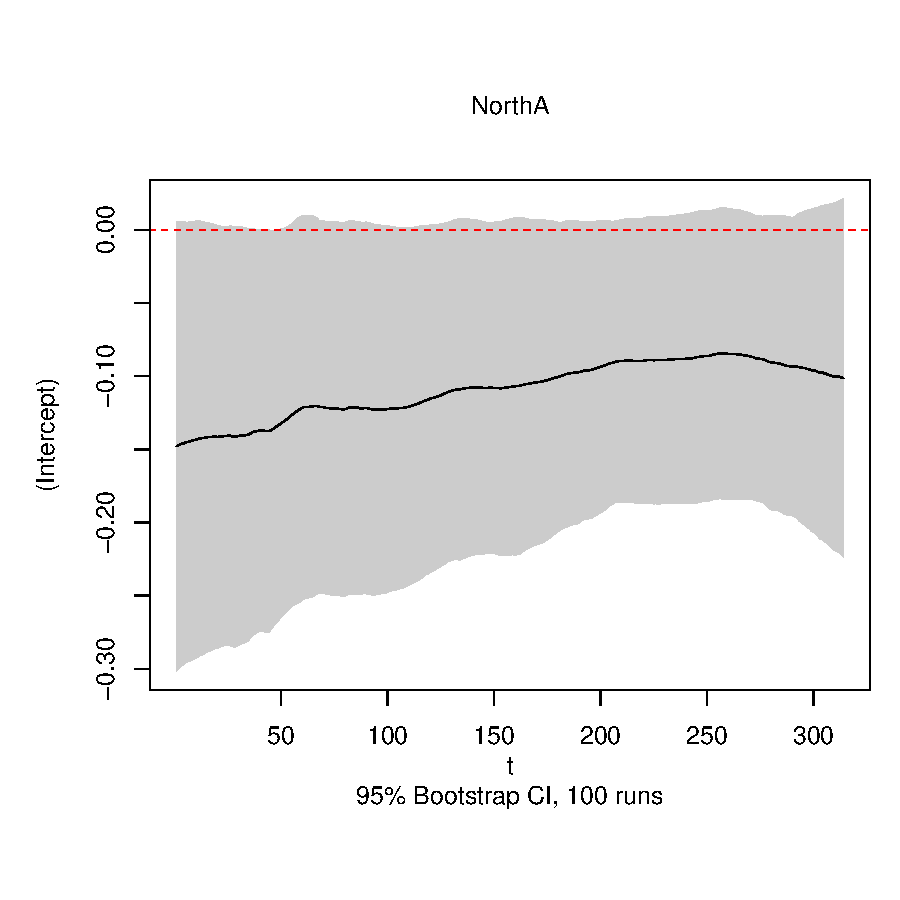
\includegraphics[page = 1, width = 0.48\textwidth]{Fig1}
\includegraphics[page = 2, width = 0.48\textwidth]{Fig1}
\includegraphics[page = 3, width = 0.48\textwidth]{Fig1}
\includegraphics[page = 4, width = 0.48\textwidth]{Fig1}
\caption{Intercept estimates of a Small/Low portfolio in the four markets (left to right, top to bottom: North America, Japan, Asia Pacific and Europe). The solid lines indicate the estimates, the grey bands are their 95\% bootstrap confidence intervals and the red dashed lines indicate zero. Only the Asia Pacific market intercepts are statistically different from zero during a large period, implying that the FF5F does not explain excess returns well for the Asia Pacific market. \label{fig:tvff5f}}
\end{figure}

The user can also choose to plot the coefficients of several variables and/or equations. Plots will be grouped by equation, with a maximum of three variables per plot. The piece of code below show how to plot the coefficients of the second and third variables from the Japan market equation, which results can be seen in Figure~\ref{fig:tvff5f2}.
%%
%% Example 2 (continued 3): tvSURE estimates plot. Application to portfolio management 
%%
\begin{Schunk}
\begin{Sinput}
> plot(TVFF5F.95, vars = c(2, 3), eqs = 2)
\end{Sinput}
\end{Schunk}

\begin{figure}[!ht]
\centering
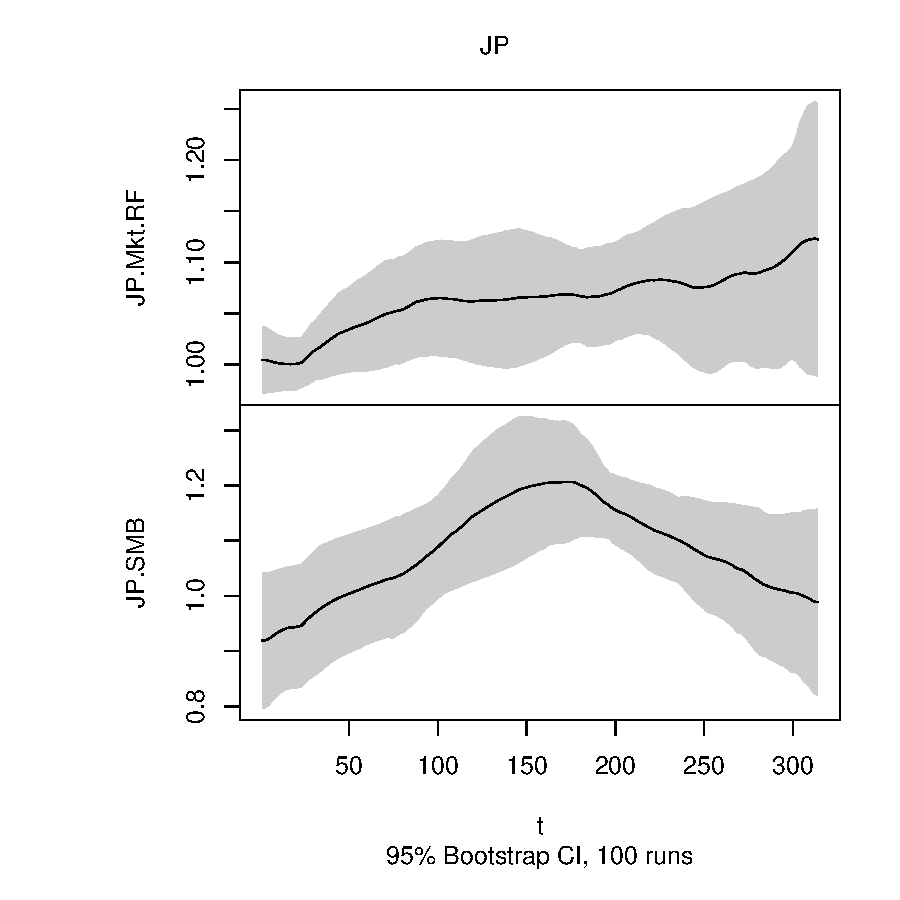
\includegraphics[width = 0.5\textwidth]{Fig2}
\caption{Coefficient estimates of excess returns on the market portfolio (JP.Mkt.RF) and JP.SMB factors for a Small/Low portfolio in the Japan market. The solid line indicates the estimates and the grey bands are their 95\% bootstrap confidence intervals. It seems that the effect of the market return over the asset return increases slightly over time, while the effect of the size premium over the asset return has an inverted U shape over the time period. \label{fig:tvff5f2}}
\end{figure}


\section{Standard usage of \code{tvPLM}}
\label{ssec:tvplm}

The \code{tvPLM} method is inspired by the \code{plm} method from the package \pkg{plm}. It converts \code{data} into an object of the class attribute \code{"pdata.frame"} using argument \code{index} to define the cross-section and time dimensions. If \code{index = NULL} (default), the two first columns of \code{data} define the dimensions. The \code{tvPLM} wraps the \code{tvRE} and \code{tvFE} methods to estimate the coefficients of time-varying panel data models.

The user can provide additional optional arguments to modify the default estimation. See section \ref{ssec:tvsure} for details on arguments \code{z}, \code{bw}, \code{est} and \code{tkernel}. Furthermore, argument \code{method} defines the estimator used. The possible choices based on package \pkg{plm} choices are: \code{"pooling"} (default), \code{"random"} and \code{"within"}.

\subsection{Application to health policy}

The income elasticity of healthcare expenditure is defined as the percentage change in healthcare expenditure in response to the percentage change in income per capita. If this elasticity is greater than one, then healthcare expenditure grows faster than income, as luxury goods do, and is driven by market forces alone. The heterogeneity of health systems among countries and time periods have motivated the use of panel data models, for example in \citet{Gerdthametal1992} who use a FE model. Recently, \citet{Casasetal2019b} have investigated the problem from the time-varying panel models perspective using the TVFE estimation. In addition to the income per capita, measured by the log GDP, the authors use the proportion of population over 65 years old, the proportion of population under 15 years old and the share of public funding of healthcare. The income elasticity estimate with a FE implemented in the \code{plm} is greater than 1, a counter-intuitive result. This issue is resolved using the TVFE implemented in the \pkg{tvReg}. The code below estimates coefficients with the parametric and semiparametric models:

%%
%% Example 3: Usage of the tvPLM formula
%%
\begin{Schunk}
\begin{Sinput}
> data("OECD")
> elast.fe <- plm::plm(lhe ~ lgdp + pop65 + pop14 + public, data = OECD, 
+                      index = c("country", "year"), model = "within")
> elast.tvfe <- tvPLM (lhe ~ lgdp + pop65 + pop14 + public, data = OECD, 
+                      index = c("country", "year"), method = "within",
+                      bw = 0.67)
> elast.fe <- confint(elast.fe)
> elast.tvfe <- confint(elast.tvfe)
\end{Sinput}
\end{Schunk}

Figure~\ref{fig:tvplm} shows the elasticity estimates using the FE and TVFE estimators. The constant coefficients model (dashed line) suggests that healthcare is a luxury good (over 1), while the time-varying coefficients (solid line) model suggests it is a value under 0.8. 

\begin{figure}[!ht]
\centering
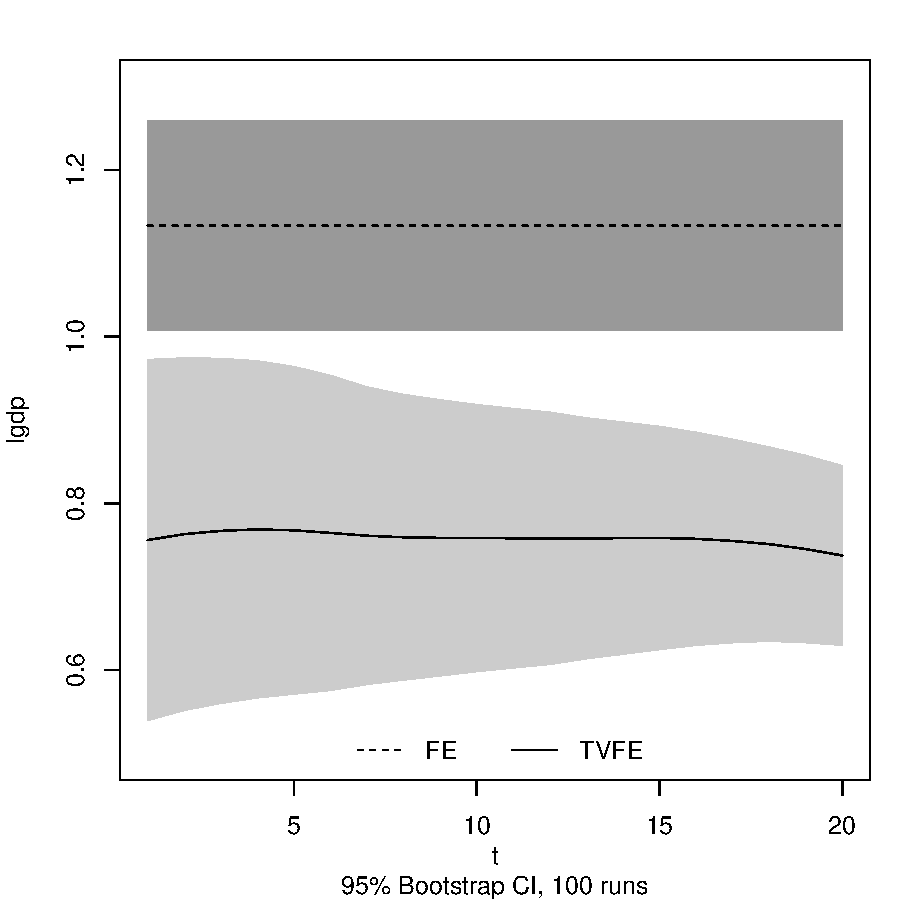
\includegraphics[width = 0.45\textwidth]{Fig3}
\caption{Comparison of income elasticity of healthcare expenditure in OECD countries. The dashed line with a dark grey band corresponds to the FE estimate and its 95\% bootstrap confidence interval, while the solid line with a light band corresponds to the TVFE estimates and their 95\% confidence intervals. There is a clear difference in the elasticity estimates of the two models. \label{fig:tvplm}}
\end{figure}


\section{Standard usage of \code{tvVAR} and \code{tvIRF}}
\label{ssec:tvvar} 
A TVVAR($p$) model is a system of time-varying autoregressive equations of order $p$. The dependent variable, \code{y}, is of the class attribute \code{"matrix"} or \code{"data.frame"} with as many columns as equations. Regressors are the same for all equations and they contain an intercept if the argument \code{type = "const"} (default) or not if \code{type = "none"}; lagged values of \code{y}; and other exogenous variables in \code{exogen}. Econometrically, the \code{tvOLS} method is called to calculate the estimates for each equation independently using one bandwidth per equation. The user can choose between automatic bandwidth selection; or entering a one value in \code{bw}, meaning that all equations will be estimated with the same bandwidth; or a vector of bandwidths, one for each equation. The \code{tvVAR} returns a \code{list} of the class attribute \code{tvvar}, which can be used to estimate the TVIRF model with the function \code{tvIRF}. 

\subsection{Application to monetary policy}

The assessment and forecast of the effects of monetary policy on macroeconomic variables, such as inflation, economic output and employment is commonly modelled using the econometric framework of VAR and interpreted by the IRF. In recent years, scholars of macroeconometrics have searched intensely for a way to include time variation in the coefficients and covariance matrix of the VAR model. The reason for this is that the macroeconomic climate evolves over time and effects of monetary policy must be identified locally rather than globally.  In the Bayesian framework, \citet{Primiceri2005} used the \citet{CarterKohn1994} algorithm to fit the TVP-VAR to this monetary policy problem. Results of the latter can be replicated with the functions in the package \pkg{bvarsv} and compared with results in the \pkg{tvReg} that fits the following TVVAR(4):
$$
\text{inf}_t = a_{t}^1 +\sum_{i=1}^4 b_{it}^ 1 \ \text{inf}_{t-i} +\sum_{i=1}^4 c_{it}^1 \ \text{une}_{t-i} +\sum_{i=1}^4 d_{it}^1\ \text{tbi}_{t-i} +u _{t}^1
$$
$$
\text{une}_t = a_{t}^2 +\sum_{i=1}^4 b_{it}^ 2 \ \text{inf}_{t-i} +\sum_{i=1}^4 c_{it}^2 \ \text{une}_{t-i} +\sum_{i=1}^4 d_{it}^2 \ \text{tbi}_{t-i} +u _{t}^2
$$
$$
\text{tbi}_t = a_{t}^3 +\sum_{i=1}^4 b_{it}^ 3 \ \text{inf}_{t-i} +\sum_{i=1}^4 c_{it}^3 \ \text{une}_{t-i} +\sum_{i=1}^4 d_{it}^3\ \text{tbi}_{t-i} +u _{t}^3.
$$

Central banks commonly regulate the money supply by changing the interest rates to keep a stable inflation growth. The R code below uses macroeconomic data from the United States, exactly the one used in \citet{Primiceri2005}, with the following three variables: inflation rate (\code{inf}), unemployment rate (\code{une}) and the three months treasury bill interest rate (\code{tbi}). For illustration, a VAR(4) model is estimated using the function \code{VAR} from the package \pkg{vars}, a TVVAR(4) model is estimated using the function \code{tvVAR} from the package \pkg{tvReg} and a TVP-VAR(4) model is estimated using  the function \code{bvar.sv.tvp} from the package \pkg{bvarsv}. Furthermore, their corresponding impulse response functions with horizon 20 are calculated to forecast how the inflation responds to a positive shock in interest rates. The TVVAR(4) can also be estimated with function \code{tvmvar} from R package \pkg{mgm}, which will give the same coefficient estimates than the \code{tvVAR} for the Gaussian kernel and same bandwidth. However, package \pkg{mgm} does not have an impulse response function and, for this reason, it is left out of the example.

%%
%% Example 4:  tvVAR estimation with coefficients as the rescaled time. Application to monetary policy. Comparison of the VAR, TVVAR and TVP-VAR models
%%
\begin{Schunk}
\begin{Sinput}
> data(usmacro, package = "bvarsv")
> VAR.usmacro <- vars::VAR(usmacro, p = 4, type = "const")
> TVVAR.usmacro <- tvVAR(usmacro, p = 4, bw = c(1.14, 20, 20), type = "const")
> TVPVAR.usmacro <- bvarsv::bvar.sv.tvp(usmacro, p = 4, pdrift = TRUE, nrep = 1000,  
+                                       nburn = 1000, save.parameters = TRUE)
\end{Sinput}
\end{Schunk}

The user can provide additional optional arguments to modify the default estimation. See Section \nameref{ssec:tvsure} to understand the usage of arguments \code{bw},   \code{tkernel},   \code{est} and  \code{singular.ok}. In addition, the function \code{tvVAR} has the following arguments:

\begin{description}
\item[Number of lags] \hfill\\
The number of lags is given by the model order set in  the argument \code{p}.
\item[Exogen variables] \hfill\\
Other exogenous variables can be included in the model using the argument \code{exogen}, which accepts a vector or a matrix with the same number of rows as the argument \code{y}.
\item[Type] \hfill\\
The default model contains an intercept (i.e., it has a mean different from zero). The user can set argument \code{type = "none"}, so the model has mean zero.
\end{description}

The variance-covariance matrix from the residuals of a TVVAR($p$) can be used to calculate the orthogonal TVIRF. The \code{plot} method for object of class attribute \code{"tvvar"} displays as many plots as equations, each plot with the fitted and residuals values as it is shown in Figure~\ref{fig:plot2} obtained with:

%%
%% Example 4 (continued): tvVAR estimation plot
%%
\begin{Schunk}
\begin{Sinput}
> plot(TVVAR.usmacro)
\end{Sinput}
\end{Schunk}

Figure~\ref{fig:plot2} shows the residuals of the inflation equation that has a mean close to zero and the fitted values are fitting the observed values closely. 

\begin{figure}[!ht]
\centering
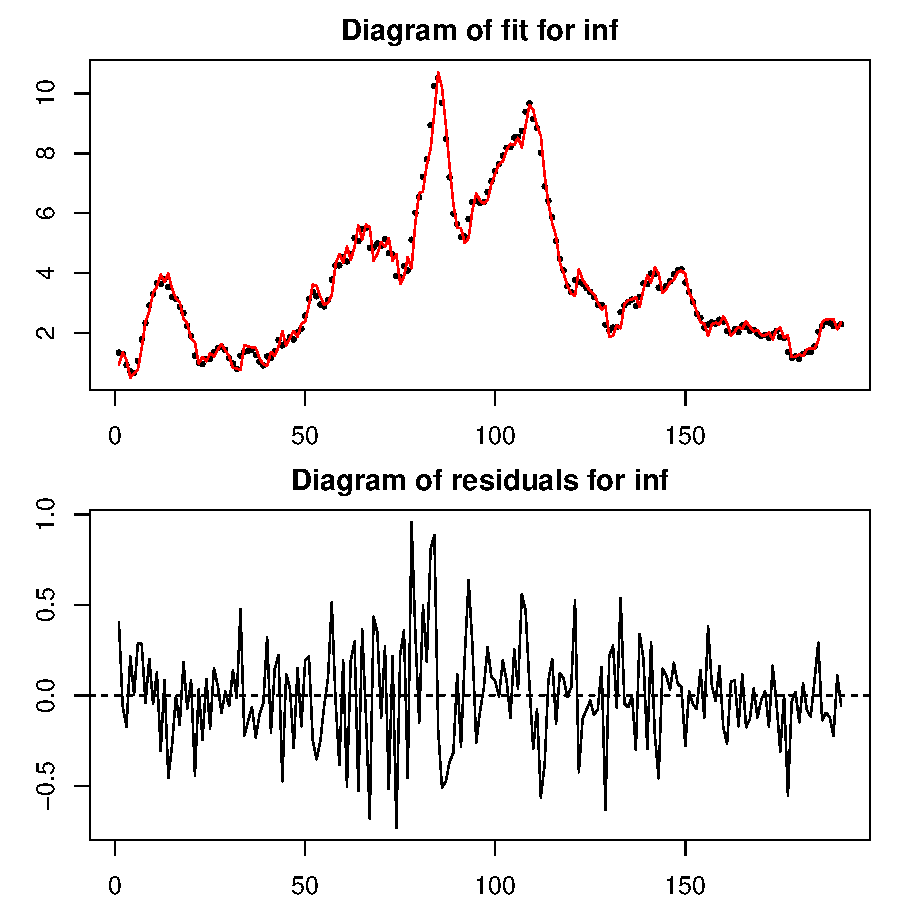
\includegraphics[page = 1, width = 0.45\textwidth]{Fig4}
\caption{Returns and fitted values of object \code{TVVAR.usmacro} for the inflation equation. The dots in the top plot represent the observed values and the red line represents the fitted values, while the black line in the bottom plot represents the returns of the estimation. The model fits the observed values well and the returns appear to have zero mean and constant variance.\label{fig:plot2}}
\end{figure}


Function \code{tvIRF} estimates the TVIRF with main argument, \code{x}, which is an object of class attribute \code{"tvvar"} returned by the function \code{tvVAR}. The user can provide additional optional arguments to modify the default estimation as explained below.

\begin{description}
\item[Impulse and response variables]\hfill\\
The user has the option to pick a subset of impulse variables and/or response variables using arguments \code{impulse} and \code{response}.
\item[Horizon]\hfill\\
The horizon of the TVIRF coefficients can be chosen by the user with argument \code{n.ahead}, the default is 10. 
\item[Orthogonal TVIRF]\hfill\\
The orthogonalised impulse response function is computed by default (\code{ortho = TRUE}). In the orthogonal case, the estimation of the variance-covariance matrix of the errors is estimated as time-varying (\code{ortho.cov = "tv"}) by default (see Section \nameref{sec:tvCov} for theoretical details). Note that the user can enter a value of the bandwidth for the variance-covariance matrix estimation in \code{bw.cov}. It is possible to use a constant variance-covariance matrix by setting \code{ortho.cov = "const"}.
\item[Cumulative TVIRF]\hfill\\
If the user desires to obtain the cumulative TVIRF values, then argument \code{cumulative} must be set to \code{TRUE}.
\end{description}

Following the previous example, the lines of code below estimate the IRF using the package \pkg{vars}, the TVP-IRF using the package \pkg{bvarsv} and the TVIRF using the package \pkg{tvReg}. 

%%
%% Example 4 (continued 2):  tvIRF estimation. Comparison with other irf estimation.
%%
\begin{Schunk}
\begin{Sinput}
> IRF.usmacro <- vars::irf(VAR.usmacro, impulse = "tbi", response = "inf", n.ahead = 20)
> TVIRF.usmacro <- tvIRF(TVVAR.usmacro, impulse = "tbi", response = "inf", n.ahead = 20)
> TVPIRF.usmacro <- bvarsv::impulse.responses(TVPVAR.usmacro, impulse.variable = 3,
+                                             response.variable = 1, draw.plot = FALSE)
\end{Sinput}
\end{Schunk}

A comparison of impulse response functions from the three estimations is plotted in Figure  \ref{fig:USMACRO}, whose R code is shown below:

%%
%% Example 4 (continued 3): graphical comparison of the irf, TVIRF and TVP-IRF for time index 150 corresponding to 1990Q2
%%
\begin{Schunk}
\begin{Sinput}
> irf1 <- IRF.usmacro$irf[["tbi"]]
> irf2 <- TVIRF.usmacro$irf[["tbi"]]
> irf3 <- TVPIRF.usmacro$irf
> ylim <- range(irf1, irf2[150,,], irf3[50,])
> plot(1:20, irf1[-1], ylim = ylim, main = "Impulse variable: tbi from 1990Q2", 
+      xlab ="horizon", ylab ="inf", type ="l", lwd = 2)
> lines(1:20, irf2[150,,-1], lty = 2, lwd = 2)
> lines(1:20, irf3[50,], lty = 3, lwd = 2)
\end{Sinput}
\end{Schunk}

Figure \ref{fig:USMACRO} displays the IRF, the TVIRF and the TVP-IRF (the two latter at time 150 in our database, which corresponds to the second quarter of 1990) for horizons 1 to 20. The IRF and TVIRF follow a similar pattern: a positive shock of one unit in the short-term interest rates (\code{tbi}) during 1990Q2 results in an initial drop in inflation during the first three months, followed by an increase for two or three months and finally in a steady decrease until it plateaus one year after. The left plot shows an increase in inflation during the first three months and a drop after. 
\begin{figure}[!ht]
\centering
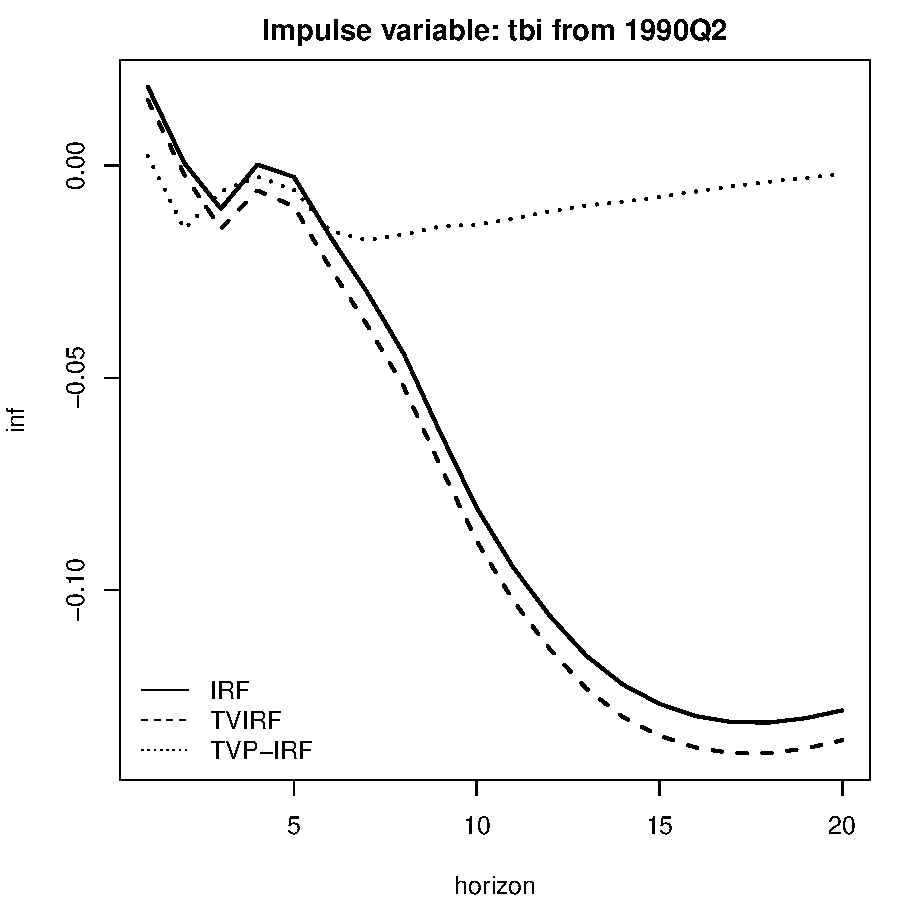
\includegraphics[width = 0.45\textwidth]{Fig5}
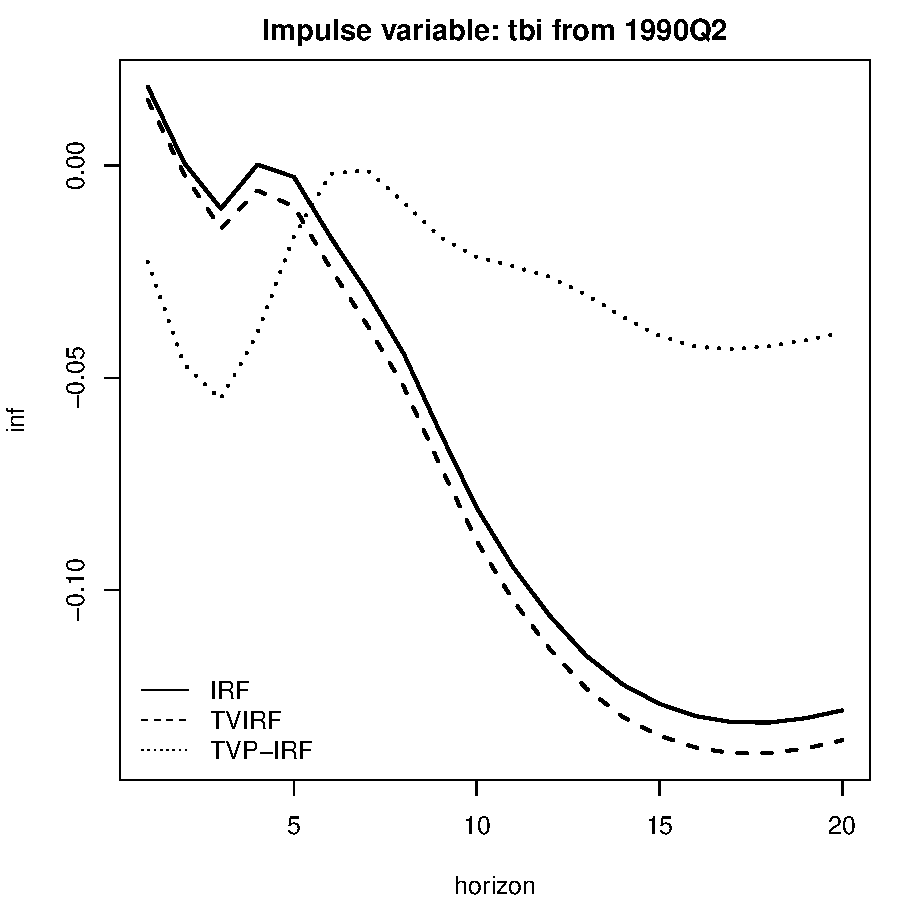
\includegraphics[width = 0.45\textwidth]{Fig6}
\caption{Estimated response of inflation (inf) to an increase in interest rates (tbi) of one unit during 1990Q2.The dashed line correspond to the IRF estimates, the solid line to the TVIRF and the dotted line to the Bayesian estimates. It appears that the Bayesian estimates are very different from those of the other two models.\label{fig:USMACRO}}
\end{figure}

The \code{confint} method is also implemented for the class attribute \code{"tvirf"}. Remember that the TVIRF model contains one impulse response function for each data time record. So, the full plot of TVIRF would have as many lines as the number of rows in the dataset. Instead, the \code{plot} method displays only one line by default, the mean value of all those impulse response functions and it issues a warning. The user can enter one or several values into argument \code{obs.index} to plot the IRF at the desire point(s) in time.


\section{Estimating a time-varying variance-covariance matrix}\label{sec:tvCov}

The time-varying variance-covariance matrix of two or more series is estimated nonparametrically in \pkg{tvReg}. Given a random process $y_{i} = (y_{i1}, \ldots, y_{iT})^\top$, such that $E(y_{it})=0$ and $E( y_{it}y_{i^{\prime }t^\prime}) = \sigma_{ii^\prime t}$ if $t=t^\prime$ and zero otherwise. Thus, the variance-covariance matrix for time $t$ is denoted by $\Sigma_t$ with elements  $\sigma_{ii^\prime, t}$ with $1 \le i, i^\prime \le N$. Given that $\Sigma_t$ is locally stationary, its local linear estimator is defined by
\begin{equation}
\mbox{vech}(\tilde {\Sigma}_\tau )=\sum_{t=1}^{T}\mbox{vech}(y_t^\top y_t)K_{h}(t-\tau){\displaystyle%
\frac{s_{2}-s_{1}\left(\tau -t\right)}{s_{0}s_{2}-s_{1}^{2}}}
\label{eq:tvSigma}
\end{equation}
where $s_j = \sum_{t=1}^T (\tau -t)^j K_b(\tau - t) $ for j = 0, 1, 2. As shown previously, $K_{b}(\cdot)$ is a symmetric kernel function heavily concentrated around the origin, $\tau =t/T$ is the focal point and $b$ is the bandwidth parameter. Note that a single bandwidth is used for all co-movements, which
ensures that $\tilde \Sigma_\tau$ is positive definite. 

The user must be aware that the local linear estimator can return non-positive definite matrices for small samples. Although the local constant estimator, calculated when $s_1 = s_2 = 1$ in (\ref{eq:tvSigma}), does not have as good asymptotic properties in the boundaries as the local linear estimator, it always provides positive definite matrices, which is a desirable property of an estimator of a variance-covariance matrix. Therefore, it is the default estimator in the function \code{tvCov}. 

The function \code{tvCov} is called by the function \code{tvIRF} to calculate the orthogonal TVIRF, and by the function \code{tvSURE} for \code{method = "tvFGLS"} to estimate the variance-covariance matrix of the error term. The function \code{tvCov} can generally be used to estimate the time-varying covariance matrix of any two or more series.


\subsection{Application to portfolio management}

\citet{AslanidisCasas2013} consider a portfolio of daily US dollar exchange rates of the Australian dollar (AUS), Swiss franc (CHF), euro (EUR), British pound (GBP), South African rand (RAND), Brazilian real (REALB) and Japanese yen (YEN), over the period from January 6, 1999 until May 7, 2010 (T = 2855 observations). This dataset contains the standarised rates after ``devolatilisation''; i.e., after standarising the rates using the GARCH(1,1) estimates of the volatility and it is available in the \pkg{tvReg} under the names of CEES. A portfolio consisting of these currencies is well diversified containing some safe haven currencies, active and liquid currencies and currencies that perform well in times of high interest rates. The estimation of the correlation matrix among these currencies is essential for portfolio management. The model is
\begin{align*}
r_{p,t} = &\omega_t^\top r_t\\
h_{p,t} = &\omega_t^\top H_t \omega_t
\end{align*}
where $r_{p,t}$ and $h_{p,t}$ are the return and variance of the portfolio at time $t$. Variable $\omega_t$ is a vector with  the weight of each currency in the portfolio strategy at time $t$. The portfolio variance-covariance matrix is denoted by $H_t$, and it may vary with time for a dynamic investment strategy. This matrix can be estimated using the function \code{tvCov} and then used in risk management, for example to calculate the Value-at-risk, denoted by VaR in the financial literature. The VaR, not be confused with the VAR, measures the level of financial risk of a portfolio, asset or firm. The VaR of an asset $X$, with distribution function $F_X$, at the confidence level $\alpha$ is defined as VaR$_\alpha = \inf\{x: F_X(x)>\alpha\}$. Commonly, the distribution function of $X$ is assumed to be Gaussian with unknown variance. In a portfolio framework, the variance-covariance matrix is estimated to calculate the VaR of a portfolio together with the portfolio weights (\code{omega} in the code below). The portfolio weights are the percentage of the total portfolio investment in each asset and can be chosen to be constant or changing over time. In the code below, weights are calculated by minimum variance at each point in time. The estimated VaR of this example portfolio is shown in Figure~\ref{fig:VaR}.

%%
%% Example 5:  Nonparametric estimation of variance-covariance matrix. Application to portfolio management
%%
\begin{Schunk}
\begin{Sinput}
> data(CEES)
> VaR <- numeric(nrow(CEES))
> Ht <- tvCov(CEES[, -1], bw = 0.12)
> e <- rep (1, ncol(CEES)-1)
> for (t in 1:nrow(CEES)){
+   omega <- solve(Ht[,,t])%*%e/((t(e)%*%solve(Ht[,,t])%*%e)[1])
+   VaR[t] <- abs(qnorm(0.05))*sqrt(max(t(omega)%*%Ht[,,t]%*%omega,0))
+ }
> plot(as.Date(CEES[, "Date"]), VaR, type ="l", xlab = "year", 
+      ylab = expression(VaR[t]), main="VaR of CEES over time")
\end{Sinput}
\end{Schunk}


\begin{figure}[!ht]
\centering
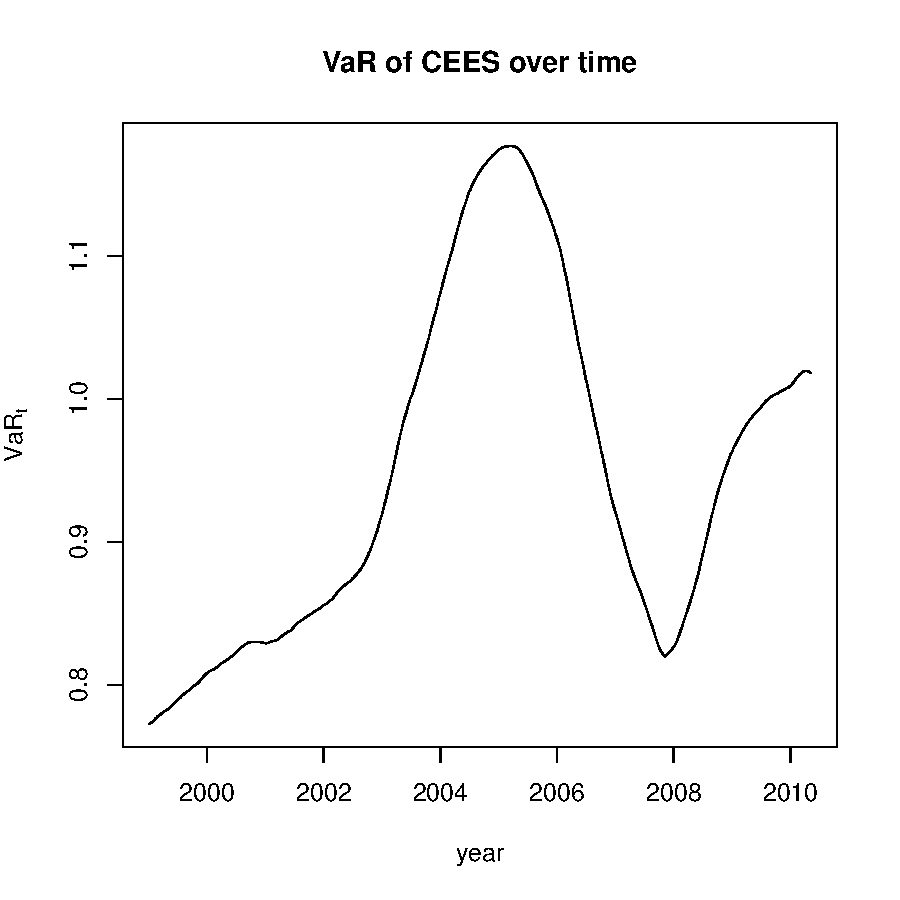
\includegraphics[width = 0.45\textwidth]{Fig7}
\caption{Dynamics of the Value-at-risk of the CEES exchange rates portfolio over time. The solid line represents the VaR. It appears that the risk of potential financial losses of this portfolio increased up to year 2005, decreasing then until 2008 and turn up again afterwards. \label{fig:VaR}}
\end{figure}


\section{Single-equation linear models with time-varying coefficients}\label{sec:single}

A varying coefficients linear model (TVLM) is generally expressed by
\begin{equation}
y_t =  x_t^\top \beta(z_t) + u_t, \ \ t= 1, \ldots, T,
\label{eq:tvlm}
\end{equation}
where $y_t$ is the response or dependent variable, $x_t = (x_{1t}, x_{2t}, \ldots, x_{dt})^\top$ is a vector of regressors at time $t$,  $\beta(z_t)$ is the vector of coefficients at time $t$ and $u_t$ is the error term which satisfies $E(u_t|x_t ) = 0$ and $E(u_t^2|x_t) = \sigma^2$. There are not enough degrees of freedom in the TVLM for a meaningful OLS estimation, but it may be estimated with the TVOLS displayed in Equation \ref{eq:tvols}. The particular case of $x_t = (y_{t-1}, y_{t-2}, \ldots, y_{t-p})$ corresponds to the time-varying autoregressive model, TVAR(p), which is also estimated with the TVOLS. 

The case of $z_t = \tau = t/T$ was firstly studied in \citet{Robinson1989} for stationary processes and generalised to nonstationary processes and correlated errors by \citet{ChangMartinezChombo2003} and \citet{Cai2007} among others. Recently, \citet{Chenetal2017} apply it to the Heterogeneous Auto-Regressive (HAR) model of \citet{Corsi2009} for the realized volatility of S\&P 500 index returns. It is a very flexible approach, but forecasts are not consistent because there is no information from the dependent variable at time $T+1$. On the other hand, the case of a random $z_t$ has been studied for iid or stationary processes by \citet{HastieTibshirani1993} and \citet{Caietal2000}; and nonstationary regressors or/and nonstationary $z_t$  have been studied by \citet{ChangMartinezChombo2003}, \citet{Caietal2009}, \citet{ZhangWue2012}, \citet{Sunetal2013}  and \citet{GaoPhillips2013}. \citet{Das2005} and \citet{xiao2013} have used the approach for instrumental variables and cointegration. In summary, this estimator is consistent and asymptotically normal for several types of dependency of $\{(x_t, z_t, u_t)\}$. 



\section{Standard usage of \code{tvLM}}
\label{ssec:tvLM}

The function \code{tvLM} fits a TVLM using the \code{tvOLS} method.  The \code{tvLM} follows the standards of the function \code{lm} with main arguments \code{formula} and \code{data}. The only mandatory argument is \code{formula}, which should be a single formula for a single-equation model. This arguments follows the standard regression \code{formula} in R. The function \code{tvLM} returns an object of the class attribute \code{tvlm}. This model is in some cases a GAM-type model which is implemented in the comprehensive and well-established \pkg{mgcv} package. The \pkg{mgcv} uses a methodology different from kernel smoothing to estimate the varying coefficients, involving splines and quasi-maximum likelihood estimation. The advantage of using kernel smoothing techniques to estimate the TVLM is that it can handle dependency and any kind of distribution in the error term. For illustration of this difference between the two packages in relation to the TVLM, the following model is generated:
\begin{equation}
y_t  = \beta_{1t} x_{1t}+ \beta_{2t} x_{2t} + u_t, \ \ t = 1, \ldots, T,
\label{eq:ex1}
\end{equation}
where $\beta_{1t}= \sin(2\pi\tau)$ and $\beta_{2t} = 2\tau$ with $\tau = t/T$ and $T = 1000$. The regressors, $x_{1t}\sim t_2$ (symmetric) and $
x_{2t} \sim \chi^2_4$, are independent of the error term, $u_t \sim \chi^2_2$ which has an exponential dependency in the covariance matrix given by $Cov(u_t, u_{t+h}) = e^{-|h|/10}$ and does not follow an exponential-family distribution. The LM, TVLM and GAM models are fitted to the data. The process generation and the fitting of a classical LM, a TVLM and a GAM are shown in the following chunk. Figure~\ref{fig:tvlm} compares the different estimates with the true $\beta_{1t}, \beta_{2t}$. As expected, the estimates from \code{lm} are constant and lie around the average of all $\beta_{1t}$ and $\beta_{2t}$, while the estimates of \code{tvLM} and \code{gam} follow the dynamics of the varying coefficients. Besides the estimates of \code{gam} fit $\beta_{1t}$ well, but not $\beta_{2t}$ although the latter is a simple linear function. This issue is caused by the autocorrelated error term with a non-exponential distribution. On the other hand, the \code{tvLM}, although it requires for a longer computation time, it is able to fit both coefficients well.


%%
%% Example 6: tvLM estimation with coefficients as function of the rescaled time
%%
\begin{Schunk}
\begin{Sinput}
> tau <- seq(1:1000)/1000
> d <- data.frame(tau, beta1 = sin(2 * pi * tau), beta2 = 2 * tau,
+                 x1 = rt(1000, df = 2), x2 = rchisq(1000, df = 4))
> error.cov <- exp(-as.matrix(dist(tau))/10)
> error <-  t(chol(error.cov)) %*% rchisq(N, df = 2)
> d <- transform(d, y = x1 * beta1 + x2 * beta2 + error)
> lm1 <- stats::lm(y ~ x1 + x2, data = d)
> TVLM1 <- tvLM(y ~ x1 + x2,  data = d, bw = 0.05, est ="ll")
> gam1 <- mgcv::gam(y ~ s(tau, by = x1) + s(tau, by = x2), data = d)
\end{Sinput}
\end{Schunk}

\begin{figure}[!ht]
\centering
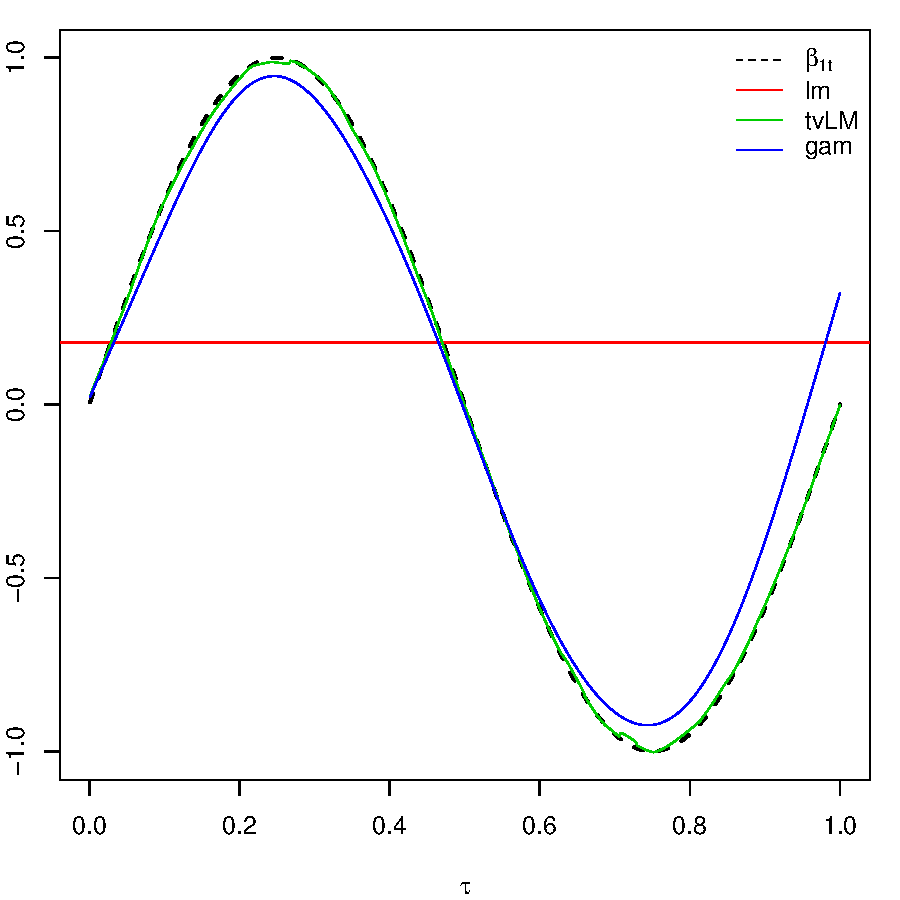
\includegraphics[page = 1, width = 0.45\textwidth]{Fig8} 
\includegraphics[page = 2, width = 0.45\textwidth]{Fig8} 
\caption{Comparison of the \code{lm}, \code{tvLM} and \code{gam} estimates of $\beta_{1t}$ and $\beta_{2t}$. The true values are plotted in black, the red lines represent the \code{lm} estimates, the green lines refer to the \code{tvLM} estimates and the blue lines represent the \code{gam} estimates. This result suggests that the TVLM is preferable for modelling non-linear varying coefficients under strong dependency.\label{fig:tvlm}}
\end{figure}

In addition to \code{formula}, the function \code{tvLM} has the arguments described in Section \nameref{ssec:tvsure} above. Also methods \code{confint}, \code{fitted}, \code{print}, \code{plot}, \code{residuals} and \code{summary} are implemented for class \code{"tvlm"}.

The \code{summary} method displays: (i) a summary of all coefficient values over the whole time period, (ii) the value of the bandwidth(s), and  (iii) a measure of goodness-of-fit, pseudo-R$^2$. The latter is printed for the class attributes \code{"tvsure"}, \code{"tvplm"}, \code{"tvvar"}, \code{"tvlm"} and \code{"tvar"} and it is calculated with the classical equation,

$$
R^2 = 1 - \frac{\sum_{t=1}^T (y_t - \hat y)^2}{\sum_{t=1}^T (y_t - \bar y)^2},
$$
where $y_t$ is the dependent variable, $\bar y$ is its mean and $\hat y_t$ are the fitted values. For multiple equation models, one pseudo-$R^2$ is calculated for each equation.


\section{Standard usage of \code{tvAR}}
\label{ssec:tvAR}
A TVAR model is a particular case of TVLM whose regressors contain lagged values of the dependent variable, \code{y}. The number of lags is given by the model order set in  the argument \code{p}. Other exogenous variables can be included in the model using the argument \code{exogen}, which accepts a vector or a matrix with the same number of rows as the argument \code{y}. An intercept is included by default unless the user enters \code{type = "none"} into the function call. Econometrically, this function also wraps the \code{tvOLS} estimator, which needs a bandwidth \code{bw} that is automatically selected when the user does not enter any number. An object of the class attribute \code{"tvar"} is returned by the function \code{tvAR}. 

The user can provide additional optional arguments to modify the default estimation of the function \code{tvAR}. See Section \nameref{ssec:tvsure} to understand the usage of  arguments \code{bw}, \code{tkernel}, \code{est} and  \code{singular.ok} and Section \nameref{ssec:tvvar} to understand the usage of argument \code{type}. In addition, the function \code{tvAR} has the following argument:

\begin{description}

\item[Coefficient restrictions] \hfill\\
An autoregressive process of order \emph{p} does not necessarily contain all the previous $p$ lags of $y_t$. Argument \code{fixed}, with the same format as in the function \code{arima} from the package \CRANpkg{stats}, permits to impose these restrictions. The order of variables in the model is: intercept (if any), lag 1, lag 2, $\ldots$, lag $p$ and exogenous variable (if any). By default, the argument \code{fixed} is a vector of \emph{NA}s with length the number of coefficients in the model. The user can enter a vector in the argument \code{fixed} with zeros in the positions corresponding to the restricted coefficients.
\end{description}


\subsection{Application to risk management}
\label{sec:RV}
The realized variance (RV) model was popularised in the financial literature by \citet{Andersenetal1998}, who show that the use of intraday data can offer an accurate forecast of daily variance. It is defined as $RV_t = \sum_{i = 1}^N r_{it}^2$, where $r_{it}$ is the price return at minute $i$ of day $t$. The autocorrelation function of the RV also shows signs of long memory in the process, which can be accounted for by the heterogeneous RV (HAR) model of \citet{Corsi2009}:
\begin{equation}
RV_t = \beta_0 + \beta_1 RV_{t-1} + \beta_2 RV_{t-1|t-5} + \beta_3 RV_{t-1|t-22} + u_{t}.
\label{eq:RV}
\end{equation}
Here, $RV_{t-1|t-k} = \frac{1}{k}\sum_{i = 1}^j RV_{t-i}$. In this model, the current $RV_t$ depends on its immediately previous value, $RV_{t-1}$, its medium-term memory factor, $RV_{t-1|t-5}$ and its long-term memory factor, $RV_{t-1|t-22}$. Basically, the HAR model may be seen as an AR(1) model with two exogenous variables. 

It is likely that changes in the business cycles affect the coefficients in (\ref{eq:RV}). \citet{Chenetal2017} coined the time-varying coefficient HAR, whose coefficients are functions of  the rescaled time period. The \code{RV} dataset contains daily variables running from January 3, 1990 until December 19, 2007 that have been computed from 5 minute intraday data from \citet{RVdata}. This period coincides with the period in \citet{Bollerslevetal2009}. The variable names in this dataset are \code{RV}, \code{RV\_lag}, \code{RV\_week}, \code{RV\_month} and \code{RQ\_lag\_sqrt} and correspond to the $RV_t$, $RV_{t-1}$, $RV_{t-1|t-5}$, $RV_{t-1|t-22}$ and $RQ_{t-1}^{1/2}$ in Model (\ref{eq:RV}). 

%%
%% Example 7: tvAR estimation with coefficients as functions of a random variable. Application to risk management
%%

\begin{Schunk}
\begin{Sinput}
> data("RV")
> RV2 <- head(RV, 2000)
> HAR <- with(RV2, arima(RV, order = c(1, 0, 0), xreg = cbind(RV_week, RV_month)))
> TVHAR<- with(RV2, tvAR(RV, p = 1, bw = 0.8, exogen = cbind(RV_week, RV_month)))
\end{Sinput}
\end{Schunk}

\citet{Bollerslevetal2016} extended the Model (\ref{eq:RV}) to control for the effect of the realized quarticity (RQ) on the relationship between the future RV and its near past values. They present the HARQ model, 

\begin{align}
RV_t = &\beta_0 + (\beta_1 + \beta_{1Q}RQ^{1/2}_{t-1}) \ RV_{t-1} +\beta_2 \ RV_{t-1|t-5} + \beta_3 \ RV_{t-1|t-22} + u_t.\label{eq:HARQ}
\end{align}
The HARQ model is a HAR model whose RV$_{t-1}$ term's coefficient is a linear function of the squared root of RQ at time $t-1$. The RQ changes over time and it will be larger during periods of more uncertainty. \citet{Casasetal2018} appreciated that the variation of this coefficient may not be linear and proposed the TVHARQ model,
\begin{equation}
RV_t = \beta_0(z_t) + \beta_1(z_t) \ RV_{t-1} + \beta_2(z_t) \ RV_{t-1|t-5} + \beta_3(z_t) \ RV_{t-1|t-22} + u_t,\label{eq:TVHAR}
\end{equation}
where the smoothing variable, $z_t=RQ^{1/2}_{t-1}$. This model is a TVAR(1) process and can be estimated with the function \code{tvAR} or with the function \code{tvLM} as it is shown in the chunk below. 

%%
%% Example 7 (continued 2): tvAR estimation with coefficients as functions of a random process, the realized quarticity. Application to risk management
%%

\begin{Schunk}
\begin{Sinput}
> HARQ <- with(RV2, lm(RV ~ RV_lag + I(RV_lag*RQ_lag_sqrt) + RV_week + RV_month))
> TVHARQ <- with(RV2, tvAR(RV, p = 1, exogen = cbind(RV_week, RV_month), 
+                          z = RQ_lag_sqrt, cv.block = 10))
\end{Sinput}
\end{Schunk}

\section{Prediction and forecast in time-varying coefficient models}
\label{sec:forecast}

Estimation is a useful tool to understand the patterns and processes hidden in known data. Prediction and forecast are the mechanisms to extend this understanding to unknown data. Although the two terms are often used indistinctively, the term prediction is broader than the term forecast which is reserved for time-series models and consists on using historical data to infer the future. For example, we speak of predicting values from a linear regression fitted to cross-sectional data and of forecasting future values from an AR(p) model.

The \emph{prediction} of the dependent variable at time $T+h$ (horizon of length $h$) in a linear regression is $\hat y_{T+h} = x_{T+h}^\top \hat \beta$ for $h\ge 1$. Future values, $x_{T+h}$, must be known to calculate the prediction. In time series, the prediction of future values has a slightly different nature and then is when we use the word \emph{forecast}. The regressors in the 1-step-ahead forecast are known, but they are effectively unknown for for longer horizons and must be forecasted first. For example, given $y_t = 5 - 0.5 y_{t-1} + u_t$ for $t = 1, \ldots, T$; the 1-step-ahead forecast is $\hat y_{T+1}^* = 5 -0.5 y_{T}$ with known $y_T$. However, the 2-step-ahead forecast is $\hat y_{T+2}^* = 5 - 0.5 \hat y_{T+1}^*$, which uses the previous forecast value, $\hat y_{T+1}^*$. 

In the \pkg{tvReg}, we refer to prediction when $z_t$ is a random variable and to forecast when $z_t = \tau$. Note that future values of the conditional variable, $z_{T+h}$, must be given for prediction. For example, the prediction problem $\hat y_{T+h} = x_{T+h}^\top \hat \beta(z_t)$ for $h\ge 1$ requires the future values $x_{T+h}$ and $z_{T+h}$. Whereas, the forecast problem $\hat y_{T+h}^* = x_{T+h}^\top \hat \beta(T+h)$ requires only the future values $x_{T+h}$. Thus, the \code{predict} and \code{forecast} methods in \pkg{tvReg} are slightly different. 


\section{Standard usage of predict and forecast}

The \code{forecast} method is implemented for the class attributes \code{"tvsure"}, \code{"tvplm"}, \code{"tvar"}, \code{"tvlm"} and \code{"tvar"}. As an example, the three days ahead forecast of model \code{TVHAR}, evaluated in Section \nameref{sec:RV} using the first 2000 values of the dataset \code{RV}, is provided in the lines of code below. This is a TVAR(1) model with two exogenous variables, \code{RV\_week} and \code{RV\_month}. The argument \code{newexogen} requires three values of these exogenous variables and variable \code{n.ahead = 3}. 

%%
%% Example 7 (continued 3):  Usage of forecast for the  model 
%%
\begin{Schunk}
\begin{Sinput}
> newexogen <- cbind(RV$RV_week[2001:2003], RV$RV_month[2001:2003])
> forecast(TVHAR, n.ahead = 3, newexogen = newexogen)
\end{Sinput}
\begin{Soutput}
[1] 2.200921e-05 2.566854e-05 2.466637e-05
\end{Soutput}
\end{Schunk}


The \code{forecast} method requires the argument \code{object}. In addition, other arguments are necessary, some of them depending on the class attribute of \code{object}.

\begin{description}

\item[Forecast horizon]
The argument \code{n.ahead} is a scalar with the forecast horizon. By default, it is set to 1.
\item[Type of forecast]
It is possible to run either an increasing window forecast (default), when the argument \code{winsize = 0} or a rolling window forecast with a window size defined in the argument \code{winsize}.

\item[newdata]\hfill\\
These arguments belong to the \code{forecast} methods and it is a \code{"vector"}, \code{"data.frame"} or \code{"matrix"} containing the new values of the regressors in the model. It is not necessary to enter the intercept. Note that this \code{newdata} does not refer to the variables in \code{exogen} which might be part of the \code{"tvar"} and \code{"tvvar"} objects. Those must be included in \code{newexogen}, if needed.

\item[newexogen]\hfill\\
This argument appears in the \code{forecast} method for the class attributes \code{"tvar"} and \code{"tvvar"} and it must be entered when the initial model contains \code{exogen} variables. It is a \code{"vector"}, \code{"data.frame"} or \code{"matrix"}.
\end{description}

The \code{predict} method is implemented for the same class attributes than the \code{forecast}. It does not require arguments \code{n.ahead} and \code{winsize}, but arguments \code{newdata} and \code{newexogen} are defined as in \code{forecast}. In addition, new values of the smoothing variable must be entered into the argument \code{newz}. This must be of the class attribute \code{"vector"} or \code{"numeric"}. The code below, predicts three future values of the \code{TVHAR} model fitted above.

%%
%% Example 7 (continued 4):  Usage of predict for the TVHARQ model 
%%
\begin{Schunk}
\begin{Sinput}
> newdata <- RV$RV_lag[2001:2003]
> newexogen <- cbind(RV$RV_week[2001:2003], RV$RV_month[2001:2003])
> newz <- RV$RQ_lag_sqrt[2001:2003]
> predict(TVHARQ, newdata, newz, newexogen = newexogen)
\end{Sinput}
\begin{Soutput}
[1] 1.741663e-05 2.402516e-05 2.088794e-05
\end{Soutput}
\end{Schunk}
 
The example below shows the usage of the \code{forecast} and \code{predict} methods for the class attribute \code{"tvsure"}.

The lines of code below forecast three values for model \code{TVOLS.fit} evaluated in Section \nameref{ssec:tvsure}. The method needs a set of new values in the argument \code{newdata}, which must have the same number of columns as the original dataset. 

%%
%% Example 2 (continued 4):  Usage of forecast for the class tvsure 
%%
\begin{Schunk}
\begin{Sinput}
> newKmenta <- data.frame(consump = c(95, 100, 102), price = c(90, 100, 103),
+                         farmPrice = c(70, 95, 103), income = c(82, 94, 115), 
+                         trend = c(21:23))
> forecast(TVOLS.fit, newdata = newKmenta, n.ahead = 3)
\end{Sinput}
\begin{Soutput}
        demand    supply
[1,]  97.92300  95.32852
[2,]  98.94076 103.48589
[3,] 105.36951 106.26576
\end{Soutput}
\end{Schunk}

In case the smoothing variable in the model is a random variable, the \code{predict} method for the class attribute \code{"tvsure"} requires also a new set of values in argument \code{newz}. The chunk below first fits a TVSURE model, \code{tvOLS.z.fit}, to the \code{Kmenta} data with the same system of equations as in the \code{TVOLS.fit}, but with random variable as the smoothing variable, which is generated as an ARMA(2,2) process. Three values of the dependent variable are predicted with the \code{predict} method. In addition to new values in the argument \code{newdata}, it requires a set of new smoothing values  in the argument \code{newz}. It returns the predicted values as a matrix with as many columns as equations in the system. 

%%
%% Example 2 (continued 5):  Usage of predict for the class tvsure
%%
\begin{Schunk}
\begin{Sinput}
> nobs <- nrow (Kmenta)
> smoothing <- arima.sim(n = nobs + 3, sd = sqrt(0.1796),
+                        list(ar = c(0.8897, -0.4858), ma = c(-0.2279, 0.2488))) 
> smoothing <- as.numeric(smoothing)
> tvOLS.z.fit <- tvSURE(system, data = Kmenta, z = smoothing[1:nobs])
> newSmoothing <- tail(smoothing, 3)
> predict(tvOLS.z.fit, newdata = newKmenta, newz = newSmoothing)
\end{Sinput}
\begin{Soutput}
       demand    supply
[1,] 100.0195  96.50136
[2,] 100.3919 105.29293
[3,] 106.1426 107.97822
\end{Soutput}
\end{Schunk}


The \code{forecast} and \code{predict} methods for the rest of the class attributes in the package follow similar patterns, and further examples can be found in the documentation of the \pkg{tvReg}.


\section{Summary}
\label{sec:recap}

Research of time-varying coefficient linear models and their estimation using kernel smoothing methods has seen a great theoretical development during the last two decades. Our own work in this field has served as inspiration to code the \pkg{tvReg} because we encounter a lack of computer applications with this functionality. Indeed, we expect that this package empowers empirical researchers working with regression and time series models with a computing tool that allows for more flexible models.

Within the R framework: (i) the \pkg{tvReg} extends functions in the R packages \pkg{systemfit}, \pkg{plm} and \pkg{vars}; (ii) it extends functions \code{lm}, \code{ar.ols} and \code{arima} to allow for varying coefficients; (iv) it complements R packages \pkg{mgcv} and \pkg{gam} for the linear regression model by providing a consistent estimator of this model for in case of dependency and a general distribution in the error term; (v) it complements R package \pkg{mgm} by adding the time-varying impulse response (TVIRF) function which is commonly used in macroeconomics; and (vi) it complements R package \pkg{bvarsv} and \pkg{MARSS} which estimate the TVVAR and TVIRF within the state-space framework. In addition, the \code{confint}, \code{fitted}, \code{forecast}, \code{plot}, \code{predict}, \code{print}, \code{resid} and \code{summary} methods are implemented for all class attributes in the \pkg{tvReg} and will allow the user to conveniently produce their research output. In any case, the user is able to produce customised plots and summaries from the returns of the functions, whose elements are accessible in the same manner as other R \code{"list"} objects.

Finally, the \pkg{tvReg} shows multiple applications in economics and finance. Specifically in asset management, portfolio management, risk management, health policy and monetary policy. The methods and datasets permit to verify results in \cite{AslanidisCasas2013, Casasetal2018, Casasetal2019a, Casasetal2019b}. Models in this paper are used in other fields too. For example, \cite{Reikard2009} uses the TVLM to forecast the wave energy flux and \cite{Haslbecketal2021} uses the TVVAR in different applications in psychology. The \pkg{tvReg} is therefore not only relevant and original but also timely.

\section*{Acknowledgements}

We thank the unknown referee for the constructive suggestions and comments on an earlier version of this paper. The first author would also like to thank her co-authors of related papers: Nektarios Aslanidis, Eva Ferreira, Jiti Gao, Stefano Grassi, Xiuping Mao, Susan Orbe, Bin Peng, Helena Veiga and Shangyu Xie whose comments, suggestions and collaboration have helped to shape this code. The first author acknowledges financial support from the European Research Council under the European Union's Horizon 2020 research and innovation program (grant no. 657182) and from the Ministerio de Econom\'ia y Competitividad (grant no. ECO2014-51914-P). The second author acknowledges financial support from the MINECO (grant no. MTM2017-82724-R), MICINN (grant no. PID2020-113578RB-I00), and from the Xunta de Galicia (Grupos de Referencia Competitiva ED431C-2020-14 and Centro de Investigaci\'on del Sistema Universitario de Galicia ED431G 2019/01), all of them through the ERDF.


\bibliography{CasasFernandez-Casal2022_Bibtex}
%\bibliographystyle{chicago}
\address{Isabel Casas\\
  Department of Economics and Finance\\
  University of Deusto\\
  Spain\\
  ORCID: 0000-0002-9063-9670\\
  \email{casasis@gmail.com}}

\address{Rub\'{e}n Fern\'andez-Casal\\
  Department of Mathematics\\
  University of A Coru\~{n}a\\
  Spain\\
  ORCID: 0000-0002-5785-3739\\
  \email{ruben.fcasal@udc.es}}

